\section{Konzeptionierung}
\label{sec:Konzeptionierung}

An den Zielen des Projektes \acs{VCL} wird deutlich, dass eine visuelle und
attraktive Darstellung des Campus Lingen entwickelt werden muss. Auf welche Art
und Weise die Realisierung des Projektziels konkret erfolgen soll, ist jedoch in
der Projektzielsetzung nicht festgelegt. Aus diesem Grund wird in der
Konzeptionierungsphase von der Projektgruppe ein Konzept für ein System
entwickelt, mit dem die zuvor definierten Ziele erreicht werden können. Die
Konzeptionierungsphase kann hierbei in die Erstellung des Grobkonzeptes, die
iterative Erarbeitung des Feinkonzeptes und die abschließende Festlegung des
Feinkonzeptes unterteilt werden. Der Ablauf der drei Teilphasen wird im
Folgenden näher erläutert.

\subsection{Grobkonzept}
\label{sec:Grobkonzept}

Das Ziel einer möglichst ansprechenden, visuellen Darstellung des
Studienstandorts Lingen und des neuen Campus unter Verwendung moderner
Webtechnologien lässt sich auf verschiedenste Weisen realisieren. 

In einem Ideenfindungsprozess hat die Projektgruppe für die Erreichung der
Projektziele geeignete Umsetzungsmöglichkeiten identifiziert. Mit der
Brainstorming-Methode werden zunächst sämtliche Ideen zur Realisierung der
Projektidee gesammelt. Die Ideensammlung, die auf diese Weise entstand, wird
anschließend gefiltert und sortiert. Die einzelnen Ideen werden zu Clustern, wie
beispielsweise "`Anforderungen aus dem Zielsystem"', "`Technologien"' und
"`Funktionalität des Systems"' zusammengefasst. Anhand dieser strukturierten
Ideensammlung werden dann konkrete Möglichkeiten zur Umsetzung der Projektidee
herausgearbeitet. Nach einer ersten Filterung der Umsetzungsmöglichkeiten hat
sich die Projektgruppe auf die folgenden drei Realiserungsalternativen geeinigt. 

\begin{description}
\item[Fotogalerie] \hfill \\
Innerhalb einer Fotogalerie soll dem Anwender der modernisierte Studienstandort
Lingen näher gebracht werden. Zu den Fotos könnten entsprechende
Informationstexte, Beschreibungen und weiterführende Links für
Studieninteressierte hinterlegt werden.

\item[Virtueller Rundgang im Stile von Google Street View] \hfill \\
Der Anwender soll interaktiv durch Panoramafotos von den Räumlichkeiten des
Campus navigieren können. Auch bei dieser Möglichkeit der Projektrealisierung
könnten dem Nutzer weiterführende Informationen zu den abgebildeten Inhalten
präsentiert werden.

\item[Virtueller Rundgang durch ein 3D-Modell] \hfill \\
Bei dieser Möglichkeit der Umsetzug soll ein 3D-Modell des gesamten
Campusgebäudes erstellt werden. Der Nutzer könnte dann virtuell duch die
modellierten Räumlichkeiten des Campus navigieren und auf diese Weise einen
Eindruck vom Studienstandort erlangen.
\end{description}

Hierbei unterscheiden sich die einzelnen Alternativen in Innovativität,
Attraktivität für den Anwender, Komplexität der Umsetzung und Grad der Zielerreichung voneinander.
Die folgende \tabelle{AlternativenVergleich} stellt die drei Varianten
hinsichtlicher der vier genannten Kritierien gegenüber.

% \begin{table}[h]
% \centering
% 
% \caption{Soll-Ist-Vergleich der Kostenplanung}%
% \label{tab:AlternativenVergleich}%
% \end{table}

\tabelleEinfg{Soll-Ist-Vergleich der Kostenplanung}{tab:AlternativenVergleich}{AlternativenVergleich}

Die vorangegangene Tabelle stellt die drei möglichen Lösungsansätze mit den Kriterien 
Innovativität, Attraktivität, Komplexität und dem Grad der Zielerreichung dar. Die 
Fotogalerie hat im Gegensatz zu den anderen Ansätzen eine geringe Innovativität. Dies 
resultiert daraus, dass eine statische Fotogalerie im Vergleich zu virtuellen Rundgängen 
innovationslos ist. Die Fotogalerie erreicht somit nur eine mittlere Attraktivität. Die 
beiden anderen Lösungsansätze besitzen aufgrund der hohen Innovativität ebenfalls eine hohe 
Attraktivität. Die Komplexität der 3D-Modellierung und des virtuellen Rundgangs sind dagegen 
höher als die der Fotogalerie, da der Einarbeitungsaufwand bei diesen beiden Ansätzen höher 
und langwieriger ist. Die Fotogalerie hat im Vergleich zu den anderen Lösungsansätzen nur 
einen geringen Grad der Zielerreichung. Die 3D-Modellierung und der virtuelle Rundgang erreichen 
hingegen einen hohen Grad der Zielerreichung, da die junge Zielgruppe durch innovative und attraktive Ansätze
effektiver angesprochen wird.

% Die Projektgruppe geht davon aus, dass vielen Nutzern innerhalb der Zielgruppe
% diese Darstellungsform durch Google Street View bereits bekannt ist. Um von den
% vorhandenen Erfahrungen der Nutzer profitieren zu können sollen bekannten
% Steuerungselemente von Google Street View adaptiert werden. Diese sind in
% \abbildung{GoogleStreetView} dargestellt.

% \begin{figure}[htb] 
% \centering
% 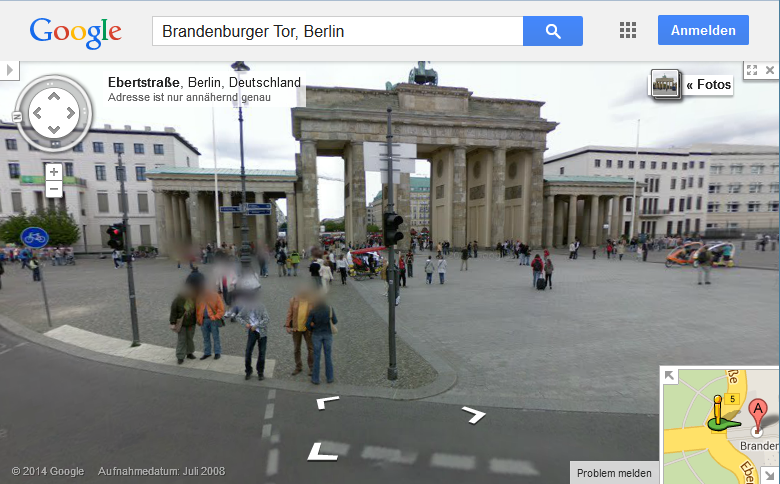
\includegraphics[width=0.7\textwidth]{GoogleStreetView.png}
% \caption[Google Street View]{Google Street View\protect\footnotemark}
% \label{fig:GoogleStreetView}
% \end{figure}
% \footnotetext{Screenshot von \url{https://maps.google.de/}}

% Die Realisierung der Projektziele wäre nach einer ersten Einschätzung der
% Projektmitglieder mit jeder der dei vorgestellten Umsetzungsmöglichkeiten
% vorstellbar. Im weiteren Verlauf der Konzeptionierungsphase soll jedoch die
% Möglichkeit herausgestellt werden, welche der Möglichkeiten für die
% Erreichung der Projektziele am besten geeignet ist.

\subsection{Iterative Erarbeitung des Feinkonzeptes}
\label{sec:ErarbeitungFeinkonzept}
\subsection{Feinkonzept}
\label{sec:Feinkonzept}

Durch die iterative Erarbeitung des Feinkonzeptes und der Genehmigung des
Projektes durch die Fakultätsleitungsrunde, wurde der Abschluss des Feinkonzepts
erfolgreich erreicht. Das endgültige Feinkonzept stellt sich folgendermaßen dar:

Die Realisierung des Projektes erfolgt mit der Umsetzungsmöglichkeit des
virtuellen Rundgangs durch den Campus im Stile von Google Street View. Dabei ist
es möglich sich virtuell durch den Campus zu bewegen. Dieses Projekt soll am
14.07.2014 abgeschlossen werden. Im Bezug auf Datenschutz werden die
Datenschutzrichtlinien beachtet, welche im Anhang x einsehbar sind. Die
Nachhaltigkeit dieses Projektes wird gewährleistet, indem die Möglichkeit
besteht, dass andere Person die Anwendung administrieren können. Dies wird über
einen Administrationsbereich realisiert, der die notwendigen Funktionen zur
Anwendungspflege bereitstellt\footnote{siehe \citet{lastenheft2013}}. Hierzu
wird ebenfalls eine Dokumentation über die Nutzung der Anwendung und der
Administration angefertigt und bei Projektabschluss übergeben. 
Nach der Erstellung und Genehmigung des Konzeptes, kann nun die
Projektdurchführung erfolgen.

%ToDo: Anhang Datenschutz verlinken

\subsection{Zielkatalog}
\label{sec:Zielkatalog}

Der Zielkatalog der Muss-Ziele besteht aus acht Zielen, von denen vier 
Ziele in einem Betatest\footnotemark\
und vier Ziel von der Projektgruppe selbst verifiziert werden. Das Ziel
gilt dabei als erreicht, wenn der festgelegte Zielindikator erfüllt wird.

\footnotetext{Am Ende des Projektes wird ein Test der Anwendung durchgeführt. Dieser Test 
beinhaltet unter anderem eine Umfrage, die zur Verifikation der oben genannte Ziel dient. 
Eine genauere Betrachtung folgt in \verweis{Projekttest}}

\textbf{Verifikation durch den Betatest:}
\begin{description}
  \item[Steigerung der Attraktivität:] Das Ziel gilt als
  erreicht, wenn innerhalb der Umfrage die Frage "`Wie bewerten Sie die durch
  die Anwendung vermittelte Attraktivität des Campus Lingen?"' von den
  Betatestern im Durchschnitt mit "`eher gut"' oder besser beantwortet wird.

  \item[Verbesserung der Präsentation von Studienprojekten:]
  Das Ziel gilt als erreicht, wenn die Frage "`Wie bewerten Sie die Präsentation
  der Studienprojekte im Vergleich zur bereits bestehenden Hochschulseite?"' von
  den Betatestern im Durchschnitt mit "`eher gut"' oder besser beantwortet wird.

  \item[Verbesserung der Präsentation aller Studiengänge:] Das Ziel gilt als erreicht, wenn
  die Frage "`Wie bewerten Sie die Art der Präsentation der einzelnen
  Studiengänge im Vergleich zur bereits bestehenden Hochschulseite?"' von den
  Betatestern im Durchschnitt mit "`eher gut"' oder besser beantwortet wird.

  \item[Verbesserung der Informationsbeschaffung:]Das Ziel gilt als erreicht, 
  wenn die Frage "`Wie bewerten Sie die
  Art der Informationsbeschaffung im Vergleich zur bereits bestehenden
  Hochschulseite?"' von den Betatestern im Durchschnitt mit "`eher gut"' oder
  besser beantwortet wird.
\end{description}

\textbf{Verifikation durch das Projektteam:}
\begin{description}
  \item[Abbildung aller Institute:]
  Kriterium bei der Bewertung ist hierbei
  die Anzahl der erstellten Fotos je Institut. Das Ziel gilt als erreicht, wenn
  mindestens 10 Bilder pro Institut in der Anwendung vorhanden sind.

  \item[Aufbau einer Administrationsoberfläche:] Das Ziel gilt als erreicht, wenn eine
  Administrationsoberfläche geschaffen wurde. Diese Administarionsoberfläche muss
  die Verwaltung der Daten der Anwendung ermöglichen. Der Datenbestand muss
  hierbei sowohl erweitert als auch gelöscht und angepasst werden können.

  \item[Entwicklung einer Anwendungsdokumentation:] Das Ziel gilt hierbei als erreicht, wenn
  für die zu realisierende Anwendung eine Dokumentation erstellt wurde. In dieser
  müssen alle relevanten Anwendungsfälle dokumentiert sein.

  \item[Erstellung unter Einhaltung der Datenschutzrichtlinien:] 
  Die in Absprache mit der Hochschule Osnabrück entstandenen
  Datenschutzrichtlinien müssen während der Erstellung beachtet werden. Es sind
  keine Abweichungen zu den Datenschutzrichtlinien erlaubt.
\end{description}

Sollten die Zielindikatoren der Muss-Ziele nicht erreicht werden können, 
so sind auch die entsprechenden Muss-Ziele des Projektes nicht erfüllt 
und das Projekt scheitert. Ein erfolgreicher
Abschluss des Projektes bedingt somit auch die Erreichug dieser Werte.

Auch wenn die Erreichung der Kann- und Soll-Ziele nicht kritisch für den
Projekterfolg ist, muss es möglich sein diese Ziele zu verifizieren. Aus diesem
Grund wurden auch diesen Zielen Zielindikatoren zugeordnet. Der komplette
Zielkatalog, in dem jedem Projektziel ein Zielindikator zugeordnet ist, kann in
\verweis{Zielkatalog} nachgeschlagen werden.

% Im nachfolgenden werden examplarisch ein Soll- und ein Kann-Ziel mit dem
% dazugehörigen Zielindikator dargestellt. Es wurden alle Muss-Ziele mit den
% dazugehörigen Indikatoren gezeigt, da diese per Definition bei einem nicht
% erreichen zum Misserfolg des Projektes führen.

% Die Erreichung des Soll-Ziels "`Verbesserung der Usability"', welches dem
% Oberziel "`Nachhaltigkeit sichern"' zugeordnet ist, wird innnerhalb des
% Betatests verifiziert. Das Ziel gilt hierbei als erreicht, wenn die Frage
% "`Konnten Sie die Anwendung intuitiv verwenden?"' von mehr als 50\% der
% Betatester mit "`Ja"' beantwortet wird.

% Ein Kann-Ziel des Oberziels "`Außendartellung des Campus Lingen
% verbessern"' ist "`Förderung eines positiven Images"'. Hierbei ist das festlegen
% eines klaren Zielindikators schwer, da eine positives Image nicht direkt auf die
% Anwendung zurückgeführt werden kann. Es handelt sich bei diesem Unterziel um ein
% qualitatives Ziel. % TODO: Begriff erklären in Fussnote? 
% Dies bedeutet das sich das erreichen des Ziels nicht dirket messen lässt. Es
% müssen Beobachtungskriterien gefunden werden die unter einer Annahme dieses Ziel
% abbilden und bewertbar sind. Die Projektgruppe entscheidet sich herbei für eine
% Frage innerhalb des Betatestfragebogens. Bei ihr wird der Tester nach dem
% potenzial der Anwendung zur Verbesserung des Images vom Campus Lingen gefragt.
% Somit kann von der Projektgruppe die Zielerreichung verifiziert werden.

% Ein detailierter Zielkatalog mit der Auflistung aller Ziele und der
% Klassifizierung nach Muss-, Soll- und Kann-Zielen mit den zugeordneten
% Zielindikatoren zur Bestimmung der Zielerreichung ist im Anhang zu finden.
\subsection{Projektrisiken}
\label{sec:Projektrisiken}


Ein Projekt in dieser größenordnung birgt einige Risiken, die innerhalb der
Durchführung eintreffen könnten und das Erreichen der Projektziels gefährden.
Solche Risiken können mittels Maßnahmenplanung im Fall des Eintritts bewältigt
werden. Jedes im Projekt erkannte Risiko wird mit einer
Eintrittswarscheinlichkeit bewertet und ein grober Plan aufgestellt, was im Fall
des Eintritts zu unternehmen ist.

Im durchzuführenden Projekt wurden folgende Risiken erkannt:

\begin{description}
\item[Ausfall der Server]
Sollte der Webserver der Anwendung ausfallen ist diese nicht mehr für die Nutzer
erreichbar und somit nicht vorhanden.
\item[Datenverlust]
Es besteht das Risiko eines Datenverlustes während der Entwicklung.
\item[Ausfall der personellen Ressourcen]
Innerhalb der Entwicklungsphase können Mitglieder des Entwicklungsteams
krankheitsbedingt ausfallen.
\item[Keine rechtzeitige Fertigstellung der Anwendung]
Es besteht das Risiko das die Anwendung nicht bis zum geplanten Übergabetermin
fertiggestellt wird.
\item[Anwendung entspricht nicht Wünschen des Kunden]
Die fertige Anwendung kann nicht den Wünschen des Kunden entsprechen.
\item[Qualität der Anwendung nicht ausreichend]
Die Anwendung entspricht nicht den Qualitätsansprüchen des Kunden.
\item[Administration der Anwendung zu komplex]
Es ist zu kompliziert die fertige Anwendung zu Administrieren.
\item[Anwendung wird gehackt und missbraucht]
Durch eine Sicherheitslücke in der Anwendung erhalten unbefugte zugriff auf die
Anwendung. 
\end{description}
%ToDo: Sind das alle Risiken ? Was ist mit Datenschutz ? Sollen diese hier
% nochmal beschrieben werden?

Die erkannten Projektrisiken sind anhand von zwei Kriterien zu kategorisieren:

\begin{itemize}
\item Warscheinlichkeit des Eintritts
\item Ausmaß des Schadens bei Eintritt 
\end{itemize}

Die Kategorisierung der erfassten Risiken wird in einer sogennanten Risikomatrix
dargestellt. An der visuell erfasst wird, wie hoch die Warscheinlichkeit eines
bestimmten Risikos ist und wie hoch der entstehende Schaden am Projekt
einzuschätzen ist.

\begin{table}[h]
\centering
\begin{tabular}{ccccl}
\hline
\multicolumn{1}{l}{} mögliches Risiko      & Wahrscheinlichkeit & Schadensausmaß
\\ \hline 
Ausfall der Server       	& Gering & Mittel  \\ \hline
Datenverlust             			& Mittel & Hoch  \\ \hline
Ausfall der personellen Ressourcen  & Mittel & Hoch \\ \hline
keine rechtzeitige Fertigstellung des Kunden & Mittel & Hoch \\ \hline
Anwendung entspricht nicht wünschen des Kunden & Gering & Hoch \\ \hline
Qualität der Anwendung nicht ausreichend & Gering & Hoch \\ \hline
Zu hoher Wartungsaufwand & Gering & Mittel \\ \hline
Anwendung wird gehackt und missbraucht & Mittel & Mittel \\ \hline
\end{tabular}
\caption{Risikomatrix}%
\label{tab:Risikomatrix}%
\end{table}

\ldots
in Arbeit 
\ldots


% Beschreibung der Auswirkungen und warum diese Warscheinlichkeit Mittel und das
% Schadensausmaß Hoch ist ??
% Risikoanalyse?!?








